\documentclass[a4paper,12pt]{article}

\usepackage{mystyle}
\usepackage{gensymb}  % \angle

\graphicspath{ {images/} }


\author{Алексеев Василий}
\title{Семинар 4}
\date{22 сентября 2022}


\begin{document}
  \maketitle
  
  \tableofcontents

  \thispagestyle{empty}
  
  \newpage
  
  \pagenumbering{arabic}
  


  \section{Скалярное произведение}
  
  \begin{definition}
    Скалярное произведение $(\bds a, \bds b)$ ненулевых\footnote{Ненулевых, чтобы можно было говорить об угле между векторами.} векторов $\bds a$ и $\bds b$ определяется следующим образом:
    \begin{equation}
      (\bds a, \bds b) \equiv |\bds a| \cdot |\bds b| \cdot \cos \phi
    \end{equation}
    где $|\bds a|$ и $|\bds b|$~---~модули векторов $\bds a$ и $\bds b$,
    а $\phi$~---~угол между векторами $\bds a$ и $\bds b$ (тот, который не превосходит $\pi$).
    В случае, если хотя бы один из пары векторов нулевой, скалярное произведение этих векторов полагается равным нулю.
  \end{definition}
  
  Отметим несколько свойств скалярного произведения:
  \begin{itemize}
    \item $(\bds a, \bds a) \geq 0$. При этом $(\bds a, \bds a) \hm= 0 \hm\Leftrightarrow \bds a \hm= \bds 0$.
    \item $(\bds a, \bds b) = (\bds b, \bds a)$~---~симметричность.
    \item Линейность по первому аргументу:
      \[
        \left\{
          \begin{aligned}
            &(\alpha \bds a, \bds c) = \alpha (\bds a, \bds c),\quad \alpha \in \RR\\
            &(\bds a + \bds b, \bds c) = (\bds a, \bds c) + (\bds b, \bds c)
          \end{aligned}
        \right.
      \]
  \end{itemize}
  
  Первые свойства следуют из определения.
  Вынесение множителя за знак скалярного произведения тоже ``в целом понятно'' (можно вывести из определения).
  Докажем последнее свойство.
  
  \begin{figure}[h]
    \centering
    
    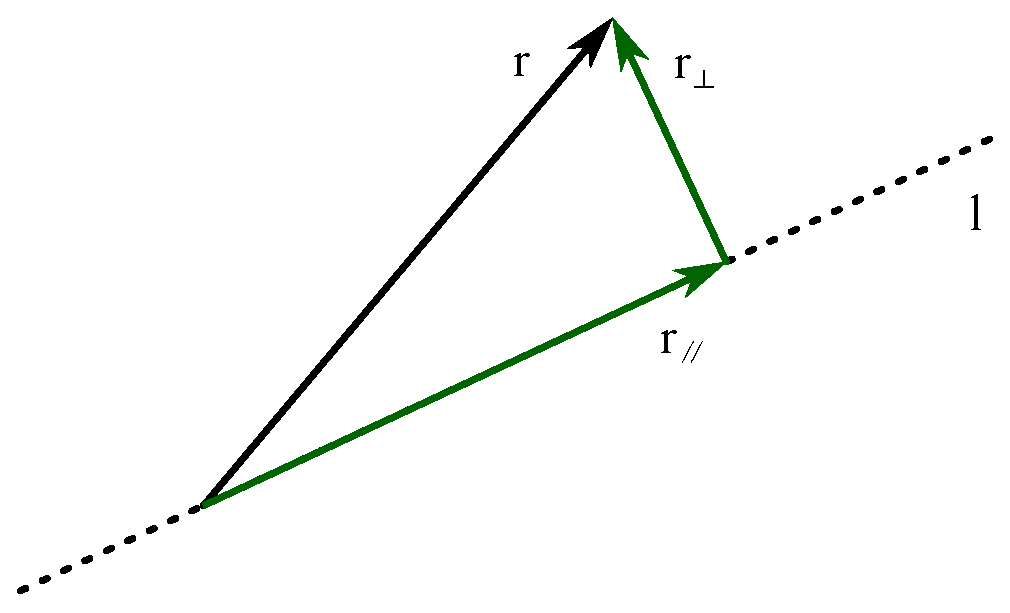
\includegraphics[width=0.5\columnwidth]{vector-projection}
    
    \caption{Ортогональная векторная проекция вектора $\bds a$ на направление, определяемое вектором $\bds c$.}
    \label{fig:vector-projection}
  \end{figure}
  
  Начнём с того, что при заданном направлении $\bds c$ любой вектор раскладывается в сумму двух (\ref{fig:vector-projection}):
  \[
    \bds a = \bds a_{\parallel} + \bds a_{\perp}
  \]
  где $\bds a_{\parallel}$~---~вектор, параллельный $\bds c$, и $\bds a_{\perp}$~---~вектор, перпендикулярный $\bds c$.
  Компонента $\bds a_{\parallel}$ называется \emph{ортогональной векторной проекцией} вектора $\bds a$ на направление, определяемое вектором $\bds c$, и может обозначаться так:
  \[
    \pi_{\bds c}(\bds a) \equiv \bds a_{\parallel}
  \]
  
  Кроме векторной проекции, есть ещё понятие скалярной проекции вектора $\bds a$ на направление вектора $\bds c$:
  \[
    \pi_{\bds c}(\bds a) \equiv |\bds a_{\parallel}| \cdot \left\{
      \begin{aligned}
        &+1 & &\mbox{если $\bds a_{\parallel} \upuparrows \bds c$}\\
        &-1 & &\mbox{если $\bds a_{\parallel} \updownarrows \bds c$}
      \end{aligned}
    \right.
  \]
  
  Будем обозначать векторную и скалярную проекции одинаково.
  (Из контекста должно быть понятно, какая имеется в виду.)

  Спроецируем теперь вектор $\bds a \hm+ \bds b$ на направление, определяемое вектором $\bds c$ (\ref{fig:sum-of-projections}):
  \[
    \pi_{\bds c}(\bds a + \bds b) = |\bds a + \bds b| \cdot \cos \phi
  \]
  где $\phi$~---~угол между вектором $\bds a \hm+ \bds b$ и вектором $\bds c$.
  
  \begin{figure}[h]
    \centering
    
    \includegraphics[width=0.5\columnwidth]{sum-of-projections}
    
    \caption{Ортогональные векторные проекции векторов $\bds a$, $\bds b$ и $\bds a \hm+ \bds b$ на направление, определяемое вектором $\bds c$.}
    \label{fig:sum-of-projections}
  \end{figure}
  
  Но проекция вектора, являющегося суммой нескольких векторов, равна сумме проекций этих векторов:
  \[
    \pi_{\bds c}(\bds a + \bds b) = \pi_{\bds c}(\bds a) + \pi_{\bds c}(\bds b)
  \]
  поэтому
  \[
    |\bds a + \bds b| \cdot \cos \phi = |\bds a| \cdot \cos \phi_1 + |\bds b| \cdot \cos \phi_2
  \]
  где $\phi_1$ и $\phi_2$~---~углы, которые образуют векторы $\bds a$ и $\bds b$ с вектором $\bds c$ (считаем, что $\bds a$, $\bds b$ и $\bds c$ ненулевые).
  Умножая обе части последнего равенства на модуль вектора $\bds c$, получаем то, что хотели доказать:
  \[
    (\bds a + \bds b, \bds c) = (\bds a, \bds c) + (\bds b, \bds c)
  \]
  \qed
  
  
  \begin{problem}[2.21]
    Длины базисных векторов $\bds e_1, \bds e_2, \bds e_3$ равны соответственно $3$, $\sqrt{2}$ и $4$.
    Углы между векторами: $\angle (\bds e_1, \bds e_2) \hm= \angle (\bds e_2, \bds e_3) \hm= 45\degree$, $\angle (\bds e_1, \bds e_3) \hm= 60\degree$.
    
    Надо вычислить длины сторон и углы параллелограмма, построенного на векторах $\bds a (1, -3, 0)$ и $\bds b (-1, 2, 1)$, заданных своими координатами в указанном базисе.
  \end{problem}
  
  \begin{solution}
    Длины сторон можно посчитать через скалярные произведения:
    \[
      |\bds a| = \sqrt{(\bds a, \bds a)},\quad |\bds b| = \sqrt{(\bds b, \bds b)}
    \]
    
    Угол между сторонами (какой-нибудь один из двух)~---~тоже:
    \[
      \cos \alpha = \frac{(\bds a, \bds b)}{|\bds a| |\bds b|}
    \]
    
    Получается, чтобы решить задачу, надо просто посчитать три скалярных произведения.
    Базис ``кривой'', поэтому считать надо ``по-честному'', отталкиваясь от базовой формулы.
    Например, модуль $\bds a$ можно посчитать так:
    \begin{equation*}
    \begin{split}
      |\bds a|^2 = (\bds a, \bds a) &= (\bds e_1 - 3 \bds e_2) \cdot (\bds e_1 - 3 \bds e_2)
      = (\bds e_1, \bds e_1) - 3 (\bds e_2, \bds e_1) - 3 (\bds e_1, \bds e_2) + 9 (\bds e_2, \bds e_2)\\
      &= \bds e_1^2 - 6 (\bds e_1, \bds e_2) + 9 \bds e_2^2
      = 9 - 18 + 18 = 9
      \Rightarrow |\bds a| = 3
    \end{split}
    \end{equation*}
    
    Аналогично, для модуля $\bds b$:
    \[
      |\bds b|^2 = (\bds b, \bds b) = (-\bds e_1 + 2 \bds e_2 + \bds e_3)^2 = \ldots = 25
    \]
    
    И скалярное $\bds a$ на $\bds b$, чтоб потом найти косинус угла:
    \[
      (\bds a, \bds b) = (\bds e_1 - 3 \bds e_2, -\bds e_1 + 2 \bds e_2 + \bds e_3) = \ldots = -12
    \]
    
    Косинус одного из углов между сторонами параллелограмма:
    \[
      \cos \alpha = \frac{-12}{3 \cdot 5} = -\frac{4}{5}
    \]
  \end{solution}
  
  
  В случае же \textbf{ортонормированного} базиса формулы с применением скалярных произведений упрощаются:
  \begin{equation}\label{eq:scalar-product-simplified}
    (\bds a, \bds b) = \sum_{i=1}^n a_i b_i
  \end{equation}
  \[
    |\bds a| = \sqrt{\sum_{i=1}^n a_i^2}
  \]
  \[
    \cos\angle(\bds a, \bds b) = \frac{\sum_{i=1}^n a_i b_i}{\sqrt{\sum_{i=1}^n a_i^2} \sqrt{\sum_{i=1}^n b_i^2}}
  \]
  
  
  \begin{problem}[2.24]
    Даны два вектора $\bds a$ и $\bds b$, причём $\bds a \hm{\not=} \bds 0$.
    Чему равна ортогональная проекция $\bds b$ на направление, определяемое вектором $\bds a$?
  \end{problem}
  
  \begin{solution}
    Скалярная ортогональная проекция $\bds b$ на направление, задаваемое $\bds a$:
    \[
      \pi_{\bds a}(\bds b) = |\bds b| \cos\angle(\bds b, \bds a)
    \]
    
    Векторная проекция:
    \[
      \bds \pi_{\bds a}(\bds b) = |\bds b| \cos\angle(\bds b, \bds a) \cdot \frac{\bds a}{|\bds a|}
    \]
    то есть скалярная проекция, умноженная на единичный вектор в направлении $\bds a$.
    Выражение можно записать по-другому, если домножить числитель и знаменатель на $|\bds a|$:
    \[
      \bds \pi_{\bds a}(\bds b) = \frac{(\bds a, \bds b)}{|\bds a|^2} \bds a
    \]
    Векторная проекция $\bds b$ сонаправлена с $\bds a$, если скалярное произведение $(\bds a, \bds b) \hm> 0$ и противоположно направлена $\bds a$ в случае, если $(\bds a, \bds b) \hm< 0$.
    Если $(\bds a, \bds b) \hm= 0$, то векторная проекция~---~нулевой вектор.
  \end{solution}


  \section{Смешанное и векторное произведения}
  
  \subsection{Ориентированное пространство}
  
  \begin{figure}[h]
    \centering
    
    \includegraphics[width=0.8\columnwidth]{two-classes}
    
    \caption{Разные классы базисов в одно-, дву- и трёхмерном пространствах.}
    \label{fig:two-classes}
  \end{figure}
  
  На прямой все векторы делятся на два класса: направленные в одну сторону вдоль прямой и в противоположную (\ref{fig:two-classes}).
  На плоскости все упорядоченные пары неколлинеарных векторов делятся на два класса: пары, где поворот от первого вектора ко второму по наименьшему углу совершается против часовой стрелки, и пары, где этот поворот совершается по часовой стрелке (\ref{fig:two-classes}).
  И в трёхмерном пространстве все упорядоченные тройки некомпланарных векторов делятся на два класса: те, где поворот от первого базисного вектора ко второму по наименьшему углу происходит против часовой стрелки, если смотреть со стороны третьего базисного вектора (\emph{правые} базисы), и те, где этот поворот происходит по часовой стрелке (\emph{левые} базисы) (\ref{fig:two-classes}).
  
  \begin{definition}
    Ориентированное пространство~---~пространство, в котором выбран класс базисов\footnote{В общем случае пространства $\RR^n$, $n \hm\geq 1$ базисы тоже образуют два класса.}.
  \end{definition}
  
  В ориентированном пространстве можно говорить о длине, площади и объёме со знаком.
  
  \begin{figure}[h]
    \centering
    
    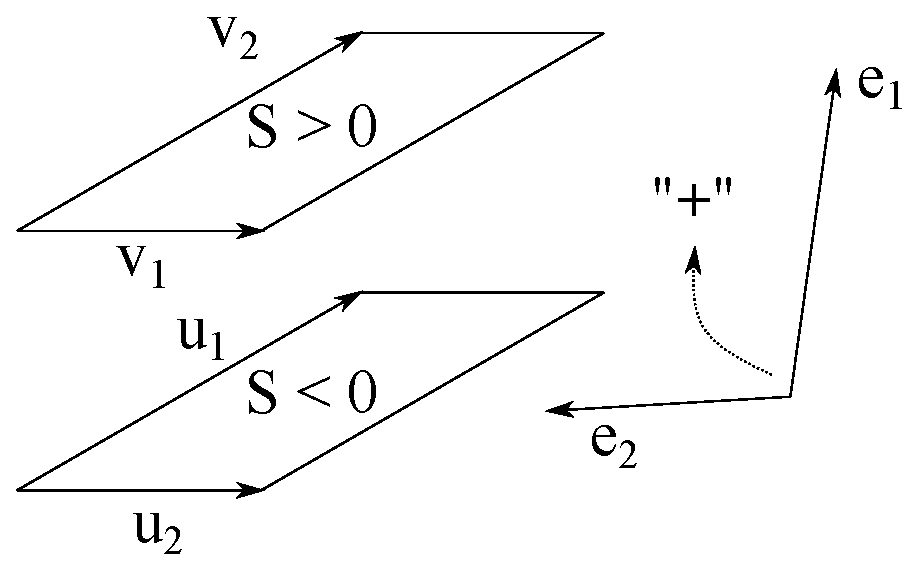
\includegraphics[width=0.5\columnwidth]{two-parallelograms}
    
    \caption{Площадь ориентированного параллелограмма.}
    \label{fig:two-parallelograms}
  \end{figure}
  
  Так, в одномерном пространстве, если рассматриваемый вектор направлен так же, как и базисы в выбранном классе, то его длина считается большей нуля.
  В противном случае~---~меньше нуля.
  В двумерном пространстве, если параллелограмм построен на \emph{упорядоченной} паре векторов $\bds a$ и $\bds b$, то его площадь со знаком $S_{\pm}$ можно считать большей нуля, если $\bds a$ и $\bds b$ образуют базис, относящийся к выбранному (положительному) классу~(\ref{fig:two-parallelograms}).
  Иначе~---~меньше нуля.
  И в трёхмерном пространстве, если параллелепипед построен на \emph{упорядоченной} тройке векторов $\bds a$, $\bds b$, $\bds c$, которые в таком же порядке образуют базис из выбранного (положительного) класса, то объём со знаком $V_{\pm}$ такого параллелепипеда будет больше нуля.
  Иначе, если тройка $\bds a$, $\bds b$, $\bds c$ не принадлежит положительному классу базисов, то объём $V_{\pm}$ параллелепипеда будет меньше нуля.
  
  \emph{В трёхмерном пространстве положительными выбраны правые базисы.}
  
  Упомянув трёхмерное пространство, стоит ещё раз вернуться к вопросу об ориентации плоскости.
  Выбор ориентации в $3$D ничего не говорит об ориентации на конкретной плоскости.
  Задать ориентацию на плоскости можно
  \begin{itemize}
    \item В $2$D~---~просто сказав, в какую сторону поворот от $\bds e_1$ к $\bds e_2$ по наименьшему углу считается положительным.
    
    \item В $3$D~---~выбрав вектор нормали $\bds n$ к плоскости.
    Тогда положительный базис на плоскости~---~тот, который с выбранной нормалью составляет положительную тройку в пространстве (порядок $\bds e_1$, $\bds e_2$, $\bds n$ или $\bds n$, $\bds e_1$, $\bds e_2$~---~не важно).
    
    \item Как в $2$D, так и в $3$D: просто выбрав упорядоченную пару неколлинеарных векторов и сказав, что этот базис положительный (тогда и все упорядоченные пары векторов из этого же класса~---~тоже положительные).
  \end{itemize}

  
  \subsection{Смешанное произведение}
  
  \begin{definition}
    В ориентированном пространстве смешанное произведение трёх некомпланарных векторов $\bds a$, $\bds b$, $\bds c$ полагается равным объёму ориентированного параллелепипеда, построенного на векторах $\bds a$, $\bds b$, $\bds c$:
    \[
      (\bds a, \bds b, \bds c) \equiv V_{\pm}(\bds a, \bds b, \bds c)
    \]
    
    Если вектора $\bds a$, $\bds b$, $\bds c$ компланарны, то их смешанное произведение полагается равным нулю.
  \end{definition}
  
  Отметим, что в смешанном произведении можно переставлять сомножители.
  Но при этом может поменяться знак смешанного произведения (если меняется класс тройки):
  \begin{equation}\label{eq:triple-change-order}
    (\bds a, \bds b, \bds c) = -(\bds b, \bds a, \bds c) = \ldots = (\bds c, \bds a, \bds b)
  \end{equation}
  
  \begin{theorem}[О связи смешанного и скалярного произведения]
    Для любой пары векторов $\bds b$, $\bds c$ существует единственный вектор $\bds d$, такой что для любого вектора $\bds a$
    \[
      (\bds a, \bds b, \bds c) = (\bds a, \bds d)
    \]
  \end{theorem}
  
  \begin{proof}
    Найдём такой вектор $\bds d$ для произвольной тройки векторов $\bds a$, $\bds b$, $\bds c$ и покажем, что он единственен и не зависит от $\bds a$.
    
    Пусть $\bds b$, $\bds c$ неколлинеарны.
    Пусть также $\bds a$, $\bds b$ и $\bds c$ некомпланарны.
    Отложим вектора $\bds a$, $\bds b$, $\bds c$ от одной точки (\ref{fig:triple-product}).
    
    \begin{figure}[h]
      \centering
      
      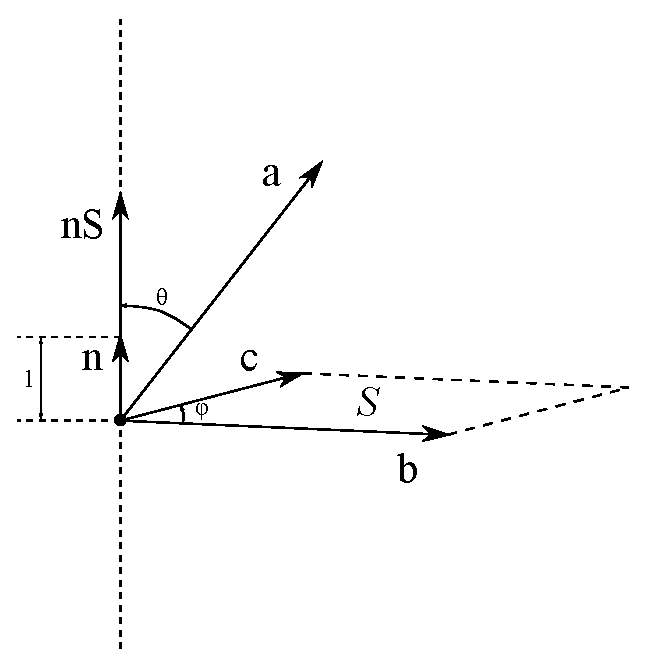
\includegraphics[width=0.5\columnwidth]{triple-product}
      
      \caption{Некомпланарные векторы $\bds a$, $\bds b$, $\bds c$; единичный вектор нормали $\bds n$ к плоскости векторов $\bds b$ и $\bds c$, такой что тройка $\bds b$, $\bds c$, $\bds n$ положительная (правая); $S$~---~площадь параллелограмма, построенного на $\bds b$ и $\bds c$.}
      \label{fig:triple-product}
    \end{figure}
  
    Рассмотрим пару векторов $\bds b$, $\bds c$.
    Отложим единичный вектор нормали $\bds n$ к плоскости векторов $\bds b$, $\bds c$ так, чтобы тройка векторов $\bds b$, $\bds c$, $\bds n$ была бы положительной.
    Площадь параллелограмма, построенного на векторах $\bds b$ и $\bds c$ (площадь без знака) равна
    \[
      S = |\bds b| \cdot |\bds c| \cdot \sin\phi
    \]
    где $\phi$~---~угол между векторами $\bds b$ и $\bds c$.
    Тогда $\bds d \hm\equiv S \hm\cdot \bds n$~---~вектор, направленный вдоль $\bds n$ и по модулю равный площади основания параллелепипеда, где лежат вектора $\bds b$, $\bds c$.
    И для объёма параллелепипеда (без знака) получаем:
    \[
      V(\bds a, \bds b, \bds c) = S \cdot \bigl||\bds a| \cdot \cos\theta\bigr|
    \]
    где $\bigl||\bds a| \cdot \cos\theta\bigr|$~---~высота.
    При этом можно заметить, что если ``убрать модуль'', то получается как раз объём со знаком:
    \[
      (\bds a, \bds d) = S \cdot |\bds a| \cdot \cos\theta = V_{\pm}(\bds a, \bds b, \bds c)
    \]
    так как именно от того, со-направлены или противоположно направлены вектора $\bds a$ и $\bds d$, зависит, будет ли $V_{\pm}$ больше или меньше нуля (тройка $\bds a$, $\bds b$, $\bds n$ по построению положительная; тройка $\bds a$, $\bds b$, $\bds c$ может быть как положительной, так и отрицательной).
    Таким образом, получаем, что
    \[
      (\bds a, \bds b, \bds c) = (\bds a, \bds d)
    \]
    
    Если же векторы $\bds a$, $\bds b$ и $\bds c$ компланарны, то объём параллелепипеда будет равен нулю, но тогда и $\bds d \hm\perp \bds a$.
    
    Если же вектора $\bds b$, $\bds c$ коллинеарны, то смешанное произведение $(\bds a, \bds b, \bds c)$ также будет равно нулю, и вектор $\bds d$ можно взять равным нулю.
    
    Покажем, что такой вектор $\bds d$, что $(\bds a, \bds b, \bds c) \hm= (\bds a, \bds d)$, $\forall \bds a$ единственен.
    Допустим противное: пусть существует вектор $\bds d_1$, такой что $(\bds a, \bds b, \bds c) \hm= (\bds a, \bds d)$ и $(\bds a, \bds b, \bds c) \hm= (\bds a, \bds d_1)$, $\forall \bds a$.
    Но тогда $(\bds a, \bds d) \hm= (\bds a, \bds d_1)$, и $(\bds a, \bds d \hm- \bds d_1) \hm= 0$.
    То есть вектор $\bds d \hm- \bds d_1$ перпендикулярен любому вектору пространства.
    Поэтому $\bds d \hm- \bds d_1 \hm= \bds 0 \hm\Rightarrow \bds d \hm= \bds d_1$.
  \end{proof}
  
  Введённый выше вектор $\bds d$ называется \emph{векторным произведением} векторов $\bds b$ и $\bds c$.
  
  \subsection{Векторное произведение}
  
  \begin{definition}
    Векторным произведением неколлинеарных векторов $\bds b$ и $\bds c$ называется вектор $\bds d$, такой что
    \begin{itemize}
      \item Модуль вектора $\bds d$ равен
      \[
        |\bds d| = |\bds b| \cdot |\bds c| \cdot \sin\alpha
      \]
      где $\alpha$~---~угол между векторами $\bds b$ и $\bds c$.
      
      \item Вектор $\bds d$ перпендикулярен как вектору $\bds b$, так и вектору $\bds c$:
      \[
        \bds d \perp \bds b,\ \bds d \perp \bds c
      \]
      
      \item Вектор $\bds d$ образует \emph{положительную тройку} $(\bds b, \bds c, \bds d)$ вместе с исходными $\bds b$ и $\bds c$\footnote{При выбранной правой ориентации пространства тройка $(\bds b, \bds c, \bds d)$ должна быть правой.}.
    \end{itemize}
    
    Если же векторы $\bds b$ и $\bds c$ коллинеарны\footnote{В этом случае не получится использовать ``связанный с положительной тройкой'' пункт определения.}, то их векторное произведение полагается равным нулю.
    
    Векторное произведение $\bds b$ и $\bds c$ может обозначаться как $[\bds b, \bds c]$ или $\bds b \hm\times \bds c$.
  \end{definition}
  
  Таким образом,
  \begin{equation}\label{eq:triple-as-scalar-and-vector}
    (\bds a, \bds b, \bds c) = (\bds a, [\bds b, \bds c])
  \end{equation}
  
  Рассмотрим некоторые свойства векторного произведения.
  
  Так, векторное произведение вектора $\bds a$ на самого себя равно нулю, так как $\bds a \hm\parallel \bds a$:
  \[
    [\bds a, \bds a] = \bds 0
  \]
  
  \begin{figure}[h]
    \centering
    
    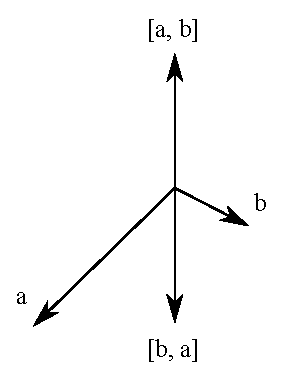
\includegraphics[width=0.25\columnwidth]{ab-ba}
    
    \caption{Векторное произведение антикоммутативно.}
    \label{fig:ab-ba}
  \end{figure}
    
  Векторное произведение обладает свойством антикоммутативности.
  Так, для любых $\bds a$ и $\bds b$
  \[
    [\bds a, \bds b] = -[\bds b, \bds a]
  \]
  так как первый и второй вектора меняются местами, и направление поворота от первого вектора ко второму меняется на противоположное (\ref{fig:ab-ba}).

  И, так же, как и скалярное произведение, векторное произведение линейно по первому аргументу:
  \[
    [\beta_1 \bds b_1 + \beta_2 \bds b_2, \bds c] = \beta_1 [\bds b_1, \bds c] + \beta_2 [\bds b_2, \bds c]
  \]
  Или, что то же самое:
  \[
    \left\{
      \begin{aligned}
        &[\beta \bds b, \bds c] = \beta [\bds b, \bds c]\\
        &[\bds b_1 + \bds b_2, \bds c] = [\bds b_1, \bds c] + [\bds b_2, \bds c]
      \end{aligned}
    \right.
  \]
  
  \begin{proof}
    Докажем это свойство.
    Надо ``в нужное время вставлять и убирать квадратные скобки'' и пользоваться линейность скалярного произведения:
    \begin{equation}
    \begin{split}
      (\bds a, [\beta_1 \bds b_1 + \beta_2 \bds b_2, \bds c])
      &\stackrel{(\ref{eq:triple-as-scalar-and-vector})}{=} (\bds a, \beta_1 \bds b_1 + \beta_2 \bds b_2, \bds c)\\
      &\stackrel{(\ref{eq:triple-change-order})}{=}         {-}(\beta_1 \bds b_1 + \beta_2 \bds b_2, \bds a, \bds c)\\
      &\stackrel{(\ref{eq:triple-as-scalar-and-vector})}{=} {-}(\beta_1 \bds b_1 + \beta_2 \bds b_2, [\bds a, \bds c])\\
      &\stackrel{\hphantom{(1)}}{=}                         {-}\beta_1(\bds b_1, [\bds a, \bds c]) - \beta_2(\bds b_2, [\bds a, \bds c])\\
      &\stackrel{(\ref{eq:triple-as-scalar-and-vector})}{=} {-}\beta_1(\bds b_1, \bds a, \bds c) - \beta_2(\bds b_2, \bds a, \bds c)\\
      &\stackrel{(\ref{eq:triple-change-order})}{=}         \beta_1(\bds a, \bds b_1, \bds c) + \beta_2(\bds a, \bds b_2, \bds c)\\
      &\stackrel{(\ref{eq:triple-as-scalar-and-vector})}{=} \beta_1(\bds a, [\bds b_1, \bds c]) + \beta_2(\bds a, [\bds b_2, \bds c])
      \stackrel{\hphantom{(1)}}{=}                         (\bds a, \beta_1[\bds b_1, \bds c] + \beta_2[\bds b_2, \bds c])
    \end{split}
    \end{equation}
  \end{proof}
  
  Теперь можно выразить векторное произведение между произвольными двумя векторами $\bds a$ и $\bds b$ пространства, которые заданы компонентами в некотором базисе $e \hm= (\bds e_1, \bds e_2, \bds e_3)$.
  Пусть
  \[
    \left\{
      \begin{aligned}
        &\bds a = a_1 \cdot \bds e_1 + a_2 \cdot \bds e_2 + a_3 \cdot \bds e_3\\
        &\bds b = b_1 \cdot \bds e_1 + b_2 \cdot \bds e_2 + b_3 \cdot \bds e_3
      \end{aligned}
    \right.
  \]
  Тогда
  \begin{equation*}
  \begin{split}
    \bds a \times \bds b
    =\; &(a_1 \cdot \bds e_1 + a_2 \cdot \bds e_2 + a_3 \cdot \bds e_3) \times (b_1 \cdot \bds e_1 + b_2 \cdot \bds e_2 + b_3 \cdot \bds e_3)\\
    =\; &(a_2 b_3 - a_3 b_2)[\bds e_2, \bds e_3] + (a_1 b_3 - a_3 b_1)[\bds e_1, \bds e_3] + (a_1 b_2 - a_2 b_1)[\bds e_1, \bds e_2]
  \end{split}
  \end{equation*}
  где в последнем переходе использовались свойство антикоммутативности векторного произведения и свойство равенства нулевому вектору векторного квадрата любого вектора.
  Полученное соотношение можно переписать в таком виде
  \begin{equation}
    [\bds a, \bds b] = \begin{vmatrix}
      [\bds e_2, \bds e_3] & [\bds e_3, \bds e_1] & [\bds e_1, \bds e_2]\\
      a_1 & a_2 & a_3\\
      b_1 & b_2 & b_3
    \end{vmatrix}
  \end{equation}
  где, отметим ещё раз, $(\bds e_1, \bds e_2, \bds e_3)$~---~произвольный базис.
  
  Если воспользоваться полученным представлением векторного произведения через компоненты векторов, подставив его в формулу (\ref{eq:triple-as-scalar-and-vector}), то получим
  \begin{equation}
    (\bds a, \bds b, \bds c) = \begin{vmatrix}
      a_1 & a_2 & a_3\\
      b_1 & b_2 & b_3\\
      c_1 & c_2 & c_3
    \end{vmatrix} \cdot (\bds e_1, \bds e_2, \bds e_3)
  \end{equation}

  Если же базис $e$ \textbf{правый ортонормированный}, то формулы упрощаются.
  Для векторного произведения:
  \begin{equation}\label{eq:vector-product-simplified}
    [\bds a, \bds b] = \begin{vmatrix}
      \bds e_1 & \bds e_2 & \bds e_3\\
      a_1 & a_2 & a_3\\
      b_1 & b_2 & b_3
    \end{vmatrix}
  \end{equation}
  и для смешанного:
  \begin{equation}\label{eq:triple-product-simplified}
    (\bds a, \bds b, \bds c) = \begin{vmatrix}
      a_1 & a_2 & a_3\\
      b_1 & b_2 & b_3\\
      c_1 & c_2 & c_3
    \end{vmatrix}
  \end{equation}
  
  
  \subsection{Задачи}
  
  Перед задачами параграфа $3$ в сборнике сказано, что базис во всех задачах, если не оговорено противное, \emph{правый ортонормированный}.
  Поэтому при решении можно будет пользоваться более простыми формулами: для векторного (\ref{eq:vector-product-simplified}), смешанного (\ref{eq:triple-product-simplified}) и скалярного (\ref{eq:scalar-product-simplified}) произведений.
  
  
  \begin{problem}[3.1(2)]
    Найти $\bds a \times \bds b$, где $\bds a(2, -1, 1)$ и $\bds b(-4, 2, -2)$.  % TODO: spacing after comma (increase)
  \end{problem}
  
  \begin{solution}
    \[
      \bds a \times \bds b = \det \begin{pmatrix}
        \bds i & \bds j & \bds k\\
        2      & -1     & 1\\
        -4     & 2      & -2
      \end{pmatrix}
      = 0 \bds i - 0 \bds j + 0 \bds k
    \]
    
    То есть $\bds a \hm\times \bds b \hm= \bds 0$.
    О чём можно бы было догадаться и сразу, просто внимательно посмотрев на координатные строки векторов $\bds a$ и $\bds b$ (они пропорциональны, а значит векторы коллинеарны).
  \end{solution}
  
  
  \begin{problem}[3.2(1)]
    Упростить выражение $[\bds a + \bds b,\ \bds a - \bds b]$.
  \end{problem}
  
  \begin{solution}
    Упрощаем, пользуясь свойствами операции векторного произведения (перемена мест~---~со сменой знака!):
    \[
      [\bds a + \bds b,\ \bds a - \bds b] = [\bds a, \bds a] - [\bds a, \bds b] + [\bds b, \bds a] - [\bds b, \bds b]
        = \bds 0 - [\bds a, \bds b] - [\bds a, \bds b] - \bds 0
        = -2 [\bds a, \bds b]
    \]
  \end{solution}
  
  
  \begin{problem}[3.8(1)]
    На векторах $\bds a(2, 3, 1)$ и $\bds b(-1, 1, 2)$, отложенных из одной точки, построен треугольник.
    Найти:
    \begin{itemize}
      \item[1)] Площадь треугольника.
      \item[2)] Длины трёх его высот.
    \end{itemize}
  \end{problem}
  
  \begin{solution}
    \leavevmode
    
    \emph{Способ 1 (``скетч'').}
    Можно бы было сделать ``по-простому'': найти длины сторон треугольника (через скалярное произведение), потом косинус угла между сторонами (тоже через скалярное произведение), потом синус, а потом и площадь треугольника.
    
    \medskip
    \emph{Способ 2.}
    А можно найти площадь с помощью векторного произведения.
    Векторное произведение $\bds a \hm\times \bds b$ даст \emph{вектор}, перпендикулярный плоскости, где лежат $\bds a$ и $\bds b$.
    Но длина этого вектора как раз будет равна удвоенной площади треугольника.
    А найти сам вектор $\bds a \hm\times \bds b$ можно с помощью формулы от компонент (\ref{eq:vector-product-simplified}):
    \[
      \bds a \times \bds b = \begin{vmatrix}
        \bds e_1 & \bds e_2 & \bds e_3\\
        2 & 3 & 1\\
        -1 & 1 & 2
      \end{vmatrix}
      = 5 \bds e_1 - 5 \bds e_2 + 5 \bds e_3
    \]
    
    Поэтому площадь будет равна:
    \[
      S_{\triangle} = \frac{\sqrt{5^2 + 5^2 + 5^2}}{2} = \frac{5 \sqrt{3}}{2}
    \]
    
    А чтобы найти высоты... видимо, всё равно придётся считать скалярные произведения)
    \[
      a = \sqrt{(\bds a, \bds a)}, \quad b = \sqrt{(\bds b, \bds b)}, \quad |\bds a - \bds b| = \sqrt{(\bds a - \bds b, \bds a - \bds b)}
    \]
    
    Дальше же высоты можно найти с помощью другой формулы площади треугольника:
    \[
      S_{\triangle} = \frac{a \cdot h_a}{2}
    \]
  \end{solution}
  
  
  \begin{problem}[3.19(3)]
    Найти смешанное произведение векторов $\bds a(2, 1, 0), \bds b(3, 4, -1), \bds c(-1, -3, 1)$.
  \end{problem}

  \begin{solution}
    \[
      (\bds a, \bds b, \bds c) = \det\begin{pmatrix}
        2 & 1 & 0\\
        3 & 4 & -1\\
        -1 & -3 & 1
      \end{pmatrix}
      = 2 - 2 + 0 = 0
    \]
    
    То есть $(\bds a, \bds b, \bds c) \hm= 0$.
    О чём можно бы было догадаться и сразу, просто внимательно посмотрев на координатные строки векторов $\bds a$, $\bds b$ и $\bds c$ (они линейно зависимы: $\bds a \hm- \bds c \hm= \bds b$~---~а значит векторы компланарны).
  \end{solution}
  
  
  \begin{problem}[3.12]
    Доказать, что для трёх неколлинеарных векторов $\bds a$, $\bds b$, $\bds c$ выполнение равенств
    \[
      [\bds a, \bds b] = [\bds b, \bds c] = [\bds c, \bds a]
    \]
    равносильно тому, что векторы $\bds a$, $\bds b$, $\bds c$ компланарны, причём
    \[
      \bds a + \bds b + \bds c = \bds 0
    \]
  \end{problem}
  
  \begin{solution}
    \leavevmode
    
    $\Leftarrow$.
    Пусть сумма векторов равна нулевому вектору.
    Тогда можно, например, выразить $\bds a$ через $\bds b$ и $\bds c$:
    \[
      \bds a = -\bds b - \bds c
    \]
    
    Подставим в векторные произведения и проверим выполнение равенств:
    \[
      [\bds a, \bds b] = [-\bds b - \bds c, \bds b]
      = -[\bds c, \bds b] = [\bds b, \bds c]
    \]
    \[
      [\bds c, \bds a] = [\bds c, -\bds b - \bds c]
      = -[\bds c, \bds b] = [\bds b, \bds c]
    \]
    
    \medskip
    
    $\Rightarrow$.
    Пусть выполнены равенства векторных произведений.
    Если известно, что, например
    \[
      [\bds a, \bds b] = [\bds b, \bds c]
    \]
    то можно это переписать как
    \[
      [\bds a + \bds c, \bds b] = \bds 0
    \]
    
    Векторы $\bds a$, $\bds b$, $\bds c$ по условию неколлинеарны, значит, ненулевые.
    Тогда из соотношения выше видно, что векторы $\bds a \hm+ \bds c$ и $\bds b$ коллинеарны, причём эту коллинеарность можно представить так:
    \[
      \bds a + \bds c = k_1 \bds b,\quad k_1 \in \RR
    \]
    
    Мы рассмотрели только одно равенство.
    Вообще же аналогичным образом можно вывести следующие соотношения:
    \[
      \left\{
        \begin{aligned}
          &\bds a + \bds c = k_1 \bds b\\
          &\bds a + \bds b = k_2 \bds c\\
          &\bds b + \bds c = k_3 \bds a
        \end{aligned}
      \right.
    \]
    
    Выразим $\bds c$ из первого соотношения:
    \[
      \bds c = k_1 \bds b - \bds a
    \]
    и подставим в третье уравнение системы.
    Получим:
    \[
      \bds b + k_1 \bds b - \bds a = k_3 \bds a \Leftrightarrow (1 + k_1) \bds b = (1 + k_3) \bds a
    \]
    
    Но $\bds a$ и $\bds b$ неколлинеарны по условию.
    Поэтому $k_1 \hm= k_3 \hm= -1$.
    Очевидно, также и $k_2 \hm= -1$.
    Раз $k_1 \hm= -1$, то
    \[
      \bds a + \bds c = -\bds b \Leftrightarrow \bds a + \bds b + \bds c = \bds 0
    \]
  \end{solution}
  
  
  \begin{problem}[3.13(2)]
    Доказать тождество (``бац минус цаб''):
    \[
      \bigl[\bds a, [\bds b, \bds c]\bigr] = \bds b (\bds a, \bds c) - \bds c (\bds a, \bds b)
    \]
  \end{problem}
  
  \begin{solution}
    \leavevmode
    
    \emph{Способ $1$ (``Стандартный'').}
    Введём базис, посчитаем левую и правую часть через компоненты векторов $\bds a$, $\bds b$ и $\bds c$, и сравним.
    
    Выберем ``хороший'' базис~---~ортонормированный.
    Пусть при этом базисный вектор $\bds e_3$ параллелен вектору $\bds c$: $\bds c \hm= \gamma_3 \bds e_3$.
    Пусть базисный вектор $\bds e_2$ лежит в плоскости векторов $\bds b$ и $\bds c$ (если они неколлинеарны, иначе~---~надо выбрать $\bds e_2$ ``просто как-нибудь'', чтоб $\bds e_3$ и $\bds e_2$ были неколлинеарны): $\bds b \hm= \beta_2 \bds e_2 \hm+ \beta_3 \bds e_3$.
    И последний вектор $\bds e_1$~---~такой, чтоб вместе с $\bds e_3$ и $\bds e_2$ образовывал правую тройку (в порядке нумерации): $\bds a \hm= \alpha_1 \bds e_1 \hm+ \alpha_2 \bds e_2 \hm+ \alpha_3 \bds e_3$.
    
    Теперь, введя базис и координаты векторов $\bds a$, $\bds b$ и $\bds c$ в этом базисе, можем начать выражать произведения между ними через их координаты:
    \[
      [\bds b, \bds c] = \det \begin{pmatrix}
        \bds e_1 & \bds e_2 & \bds e_3\\
        0        & \beta_2  & \beta_3\\
        0        & 0        & \gamma_3
      \end{pmatrix}
      = \beta_2 \gamma_3 \bds e_1
    \]
    \[
      \bigl[\bds a, [\bds b, \bds c]\bigr] = \det \begin{pmatrix}
        \bds e_1         & \bds e_2 & \bds e_3\\
        \alpha_1         & \alpha_2 & \alpha_3\\
        \beta_2 \gamma_3 & 0        & 0
      \end{pmatrix}
      = \beta_2 \gamma_3 \cdot (\alpha_3 \bds e_2 - \alpha_2 \bds e_3)
    \]
    
    И для правой части тождества, которое надо доказать:
    \[
      (\bds a, \bds c) = 0 + 0 + \alpha_3 \gamma_3 = \alpha_3 \gamma_3
    \]
    \[
      (\bds a, \bds b) = 0 + \alpha_2 \beta_2 + \alpha_3 \beta_3 = \alpha_2 \beta_2 + \alpha_3 \beta_3
    \]
    \[
      \bds b (\bds a, \bds c) - \bds c (\bds a, \bds b)
        = (\beta_2 \bds e_2 + \beta_3 \bds e_3) \cdot \alpha_3 \gamma_3 - \gamma_3 \bds e_3 \cdot (\alpha_2 \beta_2 + \alpha_3 \beta_3)
        = \beta_2 \gamma_3 \cdot (\alpha_3 \bds e_2 - \alpha_2 \bds e_3)
    \]
    
    Результаты для левой и правой частей доказываемого тождества получились одинаковыми, поэтому тождество доказано.
    
    \medskip
    
    \emph{Способ $2$ (Павел Юнкер, Б04-108, 2021\footnote{Автор конспекта впервые познакомился с таким решением, проверяя ДЗ Павла.}).}
    Приведём ещё раз тождество, которое надо доказать:
    \[
      \bigl[\bds a, [\bds b, \bds c]\bigr] = \bds b (\bds a, \bds c) - \bds c (\bds a, \bds b)
    \]
    
    Понимаем, что левая часть~---~это некоторый вектор в плоскости $(\bds b, \bds c)$.
    Причём не просто ``некоторый'', а вектор, который получается поворотом ортогональной проекции $\bds a$ на плоскость $(\bds b, \bds c)$ на $90\degree$ в направлении от $\bds c$ к $\bds b$ (\ref{fig:nonstandard-solution}).
    С правой частью уравнения пока не очень понятно (кроме того, что это тоже вектор, лежащий в плоскости векторов $\bds b$ и $\bds c$).
    
    \begin{figure}[h]
      \centering
      
      \includegraphics[width=0.5\columnwidth]{nonstandard-solution}
      
      \caption{Вектор $\bigl[\bds a, [\bds b, \bds c]\bigr]$.}
      \label{fig:nonstandard-solution}
    \end{figure}
    
    Можно ли как-то... упростить задачу?
    Перейти от исходной ``общей'' постановки к какой-нибудь другой, попроще (но так, чтоб решение более простого случая позволяло бы и исходное тождество доказать)...
    
    Зависит ли тождество от модулей векторов?
    Если один из векторов нулевой, то всё будет нулём.
    Если же векторы не нулевые, то можно просто ``отнормировать обе части тождества'' на модули векторов $\bds a$, $\bds b$ и $\bds c$.
    Таким образом, мы можем считать, что все векторы единичной длины.
    
    Зависит ли тождество от угла между векторами $\bds b$ и $\bds c$ (которые образуют базис на той плоскости, где поворачивается проекция вектора $\bds a$)?
    Допустим, $\bds b$ и $\bds c$ не перпендикулярны.
    Тода можно подобрать $k \hm\in \RR$ так, чтобы векторы $\bds b' \hm= \bds b \hm- k \bds c$ и $\bds c$ уже были перпендикулярны.
    Заменяя в исходном тождестве $\bds b$ на $\bds b' \hm+ k \bds c$, получаем... точно такое же тождество, но с вектором $\bds b'$ вместо $\bds b$!
    Таким образом, мы можем считать, что векторы $\bds b$ и $\bds c$ перпендикулярны.
    
    Теперь понятен смысл правой части тождества: это ортогональная проекция $\bds a$ на плоскость $(\bds b, \bds c)$, но повёрнутая на $90\degree$ в направлении от $\bds c$ к $\bds b$.
    (Выражения $(\bds a, \bds c)$ и $(\bds a, \bds b)$ дают ортогональные проекции на $\bds c$ и $\bds b$ соответственно.
    Поэтому ортогональная проекция на плоскость \emph{до поворота}: $\bds b (\bds a, \bds b) \hm+ \bds c (\bds a, \bds c)$.)
    То есть это ровно то же самое, что даёт левая часть!
    
    Тождество доказано.
  \end{solution}
  
  
  \begin{problem}[3.15]
    Даны векторы $\bds a$ и $\bds b$, такие что
    \[
      \left\{
        \begin{aligned}
          &\bds a \not= \bds 0\\
          &(\bds a, \bds b) = 0
        \end{aligned}
      \right.
    \]
    
    Надо выразить через $\bds a$ и $\bds b$ какой-нибудь вектор $\bds x$, удовлетворяющий уравнению
    \[
      [\bds x, \bds a] = \bds b
    \]
  \end{problem}
  
  \begin{solution}
    Из условия следует, что либо $\bds b \hm{\not=} \bds 0$ и $\bds b \hm\perp \bds a$, либо $\bds b \hm= \bds 0$.
    Будем пока считать, что $\bds b$ не равен нулю (\ref{fig:ba-equals-x}).
    
    \begin{figure}[h]
      \centering
      
      \includegraphics[width=0.5\columnwidth]{ba-equals-x}
      
      \caption{$[\bds x, \bds a] = \bds b$.}
      \label{fig:ba-equals-x}
    \end{figure}
    
    Так как $[\bds x, \bds a] \hm= \bds b$, то $\bds x \hm\perp \bds b$ и $|\bds x| \hm\cdot |\bds a| \hm\cdot \sin\alpha \hm= |\bds b|$, где $\alpha \hm= \angle{(\bds x, \bds a)}$.
    То есть
    \[
      |\bds x| \sin\alpha = \frac{|\bds b|}{|\bds a|}
    \]
    
    Пусть решению $\bds x_0$ соответствует угол $\alpha \hm= \dfrac{\pi}{2}$, то есть вектор $\bds x_0$ перпендикулярен как $\bds b$, так и $\bds a$.
    Тогда $\bds x_0$ сонаправлен $[\bds a, \bds b]$ (векторное произведение~---~именно в таком порядке) (\ref{fig:ba-equals-x}).
    И найти $\bds x_0$ можно как
    \[
      \bds x_0 = \underbrace{\frac{[\bds a, \bds b]}{\bigl|[\bds a, \bds b]\bigr|}}_{\mbox{``направление''}} \cdot \underbrace{\frac{|\bds b|}{|\bds a|}}_{\mbox{модуль}}
      = \frac{[\bds a, \bds b]}{|\bds a|^2}
    \]
    
    Если $\bds b \hm= 0$, то по формуле получаем $\bds x_0 \hm= \bds 0$, что тоже является решением уравнения.
  \end{solution}
  
  
  \begin{problem}[3.20(1)]
    Проверить, компланарны ли векторы, заданные своими координатами в произвольном базисе:
    \[
      \bds a(2, 3, 5),\quad \bds b(7, 1, -1),\quad \bds c(3, -5, -11)
    \]
  \end{problem}
  
  \begin{solution}
    \leavevmode
    
    \emph{Способ $1$ (``скетч'').}
    Компланарность трёх векторов равносильна их линейной зависимости.
    Поэтому можно бы было составить линейную комбинацию векторов $\bds a$, $\bds b$, $\bds c$ и приравнять её нулю.
    Если бы получилось найти нетривиальное решение (коэффициенты перед векторами), то система бы была линейно зависимой.
    В противном случае~---~линейно независимой.
    
    \medskip
    
    \emph{Способ $2$.}
    Компланарность трёх векторов также равносильна тому, что объём параллелепипеда, построенного на этих векторах, равен нулю.
    А объём можно посчитать через смешанное произведение.
    Если обозначить исходный базис как $e \hm= (\bds e_1, \bds e_2, \bds e_3)$, то объём параллелепипеда со знаком будет равен:
    \[
      V_{\pm}(\bds a, \bds b, \bds c) = \begin{vmatrix}
        2 & 3 & 5\\
        7 & 1 & -1\\
        3 & -5 & -11
      \end{vmatrix} (\bds e_1, \bds e_2, \bds e_3)
    \]
    
    Смешанное $(\bds e_1, \bds e_2, \bds e_3)$ точно не ноль.
    Но определитель даст ноль, поэтому и объём ноль, и векторы компланарны.
  \end{solution}
  
  
  \section{Дополнение}
  
  \subsection{Ещё пара задач про скалярное произведение}
  
  \begin{problem}[2.21 (Другой способ)]
    Длины базисных векторов $\bds e_1, \bds e_2, \bds e_3$ равны соответственно $3$, $\sqrt{2}$ и $4$.
    Углы между векторами: $\angle (\bds e_1, \bds e_2) \hm= \angle (\bds e_2, \bds e_3) \hm= 45\degree$, $\angle (\bds e_1, \bds e_3) \hm= 60\degree$.
    
    Надо вычислить длины сторон и углы параллелограмма, построенного на векторах $\bds a (1, -3, 0)$ и $\bds b (-1, 2, 1)$, заданных своими координатами в указанном базисе.
  \end{problem}
  
  \begin{solution}
    Мы ``умеем'' считать скалярное произведение в ``хорошем'' базисе (ортонормированном).
    Поэтому, чем считать всё в ``кривом'' базисе, можно... ``починить'' этот самый базис, и формулы для скалярного произведения будут простыми.
    
    Как ``починить'' базис $(\bds e_1, \bds e_2, \bds e_3)$?
    Можно отнормировать векторы.
    Но базис всё равно останется ``кривым''.
    Нам ещё надо как-то ``повернуть'' базисные векторы, чтобы они стали перпендикулярны...
    
    Но вместо того, чтоб пытаться последовательно из старого базиса получить новый, мы можем сразу \emph{выбрать подходящий ортонормированный новый базис}, а потом просто найти нужную матрицу перехода, чтобы пересчитать компоненты векторов $\bds a$ и $\bds b$.
    
    \begin{figure}[h]
      \centering
      
      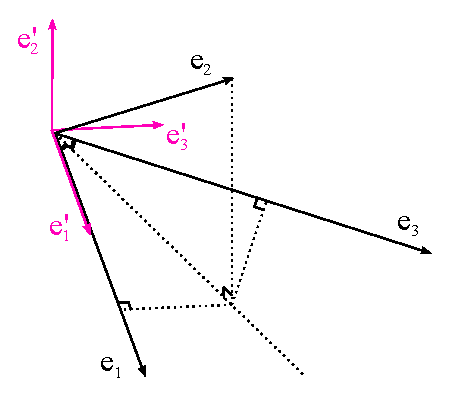
\includegraphics[width=0.5\columnwidth]{making-bew-basis}
      
      \caption{Выбор нового базиса $e'$ (ортонормированного).}
      \label{fig:making-bew-basis}
    \end{figure}
    
    Вектор $\bds e_2$ образует одинаковые углы с $\bds e_1$ и $\bds e_3$.
    Поэтому будем смотреть на исходный базис так, словно $\bds e_1$ и $\bds e_3$ лежат в горизонтальной плоскости, а $\bds e_2$ из неё выходит (\ref{fig:making-bew-basis}).
    Направим $\bds e_1'$ вдоль $\bds e_1$.
    Вектор $\bds e_3'$ выберем так, чтоб он был в той же горизонтальной плоскости, и чтоб поворот от $\bds e_1'$ к $\bds e_3'$ совершался в ту же сторону (по или против часовой стрелки), что и поворот от $\bds e_1$ к $\bds e_3$.
    Вектор $\bds e_2'$ направим в ту же сторону (в то же полупространство), что и $\bds e_2$.
    Новый базис $e'$ построен.
    
    От чего к чему искать матрицу перехода\footnote{Возможно, в такой постановке вопрос лишний, потому что раскладывать векторы $e'$ по $e$ представляется проблематичным.}?
    Если $e \hm= e' S'$, то $\bds x' \hm= S' \bds x$.
    То есть чтобы понять, как векторы раскладываются в новом (``хорошем'') базисе, надо понять, как векторы старого (``плохого'') базиса выражаются в новом базисе.
    
    Удачный выбор $e'$ позволяет ``не очень сложно'' (``из геометрии'') получить указанную матрицу перехода $S'$ (столбцы которой~---~координаты векторов ``плохого'' базиса в ``хорошем''\footnote{Осторожно: обычно всегда искали матрицу перехода от ``старого'' базиса к ``новому'', а тут наоборот.}):
    \[
      S' = \begin{pmatrix}
        3 & 1 & 2\\
        0 & \sqrt{2/3} & 0\\
        0 & 1/\sqrt{3} & 2\sqrt{3}
      \end{pmatrix}
    \]
    
    Тогда координаты векторов в ``хорошем'' базисе:
    \[
      \bds a' = S' \bds a = \begin{pmatrix}
        3 & 1 & 2\\
        0 & \sqrt{2/3} & 0\\
        0 & 1/\sqrt{3} & 2\sqrt{3}
      \end{pmatrix} \begin{pmatrix}
        1 \\ -3 \\ 0
      \end{pmatrix}
      = \begin{pmatrix}
        0 \\ -\sqrt{6} \\ -\sqrt{3}
      \end{pmatrix}
    \]
    \[
      \bds b' = S' \bds b = \begin{pmatrix}
        3 & 1 & 2\\
        0 & \sqrt{2/3} & 0\\
        0 & 1/\sqrt{3} & 2\sqrt{3}
      \end{pmatrix} \begin{pmatrix}
        -1 \\ 2 \\ 1
      \end{pmatrix}
      = \begin{pmatrix}
        1 \\ 2\sqrt{2}/\sqrt{3} \\ 8/\sqrt{3}
      \end{pmatrix}
    \]
    
    Скалярное произведение (тех же векторов, но с координатами в ``хорошем'' базисе):
    \[
      (\bds a, \bds b) = 0 \cdot 1 + \left(-\sqrt{6}\right) \cdot \left(2\sqrt{2}/\sqrt{3}\right) + \left(-\sqrt{3}\right) \cdot 8/\sqrt{3} = -12
    \]
  \end{solution}
  
  
  \begin{problem}[2.22]
    Длины базисных векторов $\bds e_1, \bds e_2, \bds e_3$ равны соответственно $1$, $1$ и $2$.
    Углы между векторами: $\angle (\bds e_1, \bds e_2) \hm= 90\degree$, $\angle (\bds e_1, \bds e_3) \hm= \angle (\bds e_2, \bds e_3) \hm= 60\degree$.
    
    Надо найти площадь параллелограмма, построенного на векторах $\bds a (-1, 0, 2)$ и $\bds b (2, -1, 1)$.
  \end{problem}
  
  \begin{solution}
    Базис не ортонормированный, поэтому скалярные произведения надо будет считать ``по-честному''.
    
    Модуль вектора $\bds a$:
    \[
      |\bds a|^2 = (\bds a, \bds a) = (-\bds e_1 + 2\bds e_3)(-\bds e_1 + 2\bds e_3)
        = (\bds e_1, \bds e_1) - 4 (\bds e_1, \bds e_3) + 4 (\bds e_3, \bds e_3)
        = 1 - 4 + 16 = 13
    \]
    
    Аналогично для вектора $\bds b$:
    \[
      |\bds b|^2 = (\bds b, \bds b) = (2\bds e_1 - \bds e_2 + \bds e_3)(2\bds e_1 - \bds e_2 + \bds e_3)
        = \ldots = 11
    \]
    
    Косинус угла между векторами $\bds a$ и $\bds b$:
    \[
      \cos\angle(\bds a, \bds b) = \frac{(\bds a, \bds b)}{|\bds a| \cdot |\bds b|}
        = \frac{(-\bds e_1 + 2\bds e_3) \cdot (2\bds e_1 - \bds e_2 + \bds e_3)}{\sqrt{13} \cdot \sqrt{11}}
        = \ldots = \frac{7}{\sqrt{13} \cdot \sqrt{11}}
    \]
    
    Поэтому синус угла будет равен:
    \[
      \sin\angle(\bds a, \bds b) = \sqrt{1 - \frac{49}{13 \cdot 11}}
    \]
    
    И площадь параллелограмма:
    \[
      S = |\bds a| \cdot |\bds b| \cdot \sin\angle(\bds a, \bds b) = \sqrt{13} \cdot \sqrt{11} \cdot \sqrt{1 - \frac{49}{13 \cdot 11}} = \sqrt{94}
    \]
  \end{solution}
  
  
  \begin{problem}[Про точку пересечения высот в треугольнике]
    Используя скалярное произведение, доказать, что в любом треугольнике высоты пересекаются в одной точке.
  \end{problem}
  
  \begin{solution}
    Пусть в $\triangle ABC$ высоты $AA_1$ и $BB_1$ пересекаются в точке $O$ (\ref{fig:triangle-with-two-hs}).
    Тогда надо показать, что прямая $CO \hm\perp AB$.
    
    \begin{figure}[h]
      \centering
    
      \includegraphics[width=0.5\columnwidth]{triangle-with-two-hs}
    
      \caption{Точка $O$ пересечения двух высот $AA_1$ и $BB_1$ в $\triangle ABC$.}
      \label{fig:triangle-with-two-hs}
    \end{figure}
  
    Так как $AO \hm\perp BC$ и $BO \perp AC$, то
    \[
      \left\{
        \begin{aligned}
          &\vv{OA} \cdot \vv{BC} = 0\\
          &\vv{OB} \cdot \vv{AC} = 0
        \end{aligned}
      \right.
    \]
    \[
      \left\{
        \begin{aligned}
          &\vv{OA} \cdot (\vv{OC} - \vv{OB}) = 0\\
          &\vv{OB} \cdot (\vv{OC} - \vv{OA}) = 0
        \end{aligned}
      \right.
    \]
    \[
      \left\{
        \begin{aligned}
          &\vv{OA} \cdot \vv{OC} = \vv{OA} \cdot \vv{OB}\\
          &\vv{OB} \cdot \vv{OC} = \vv{OB} \cdot \vv{OA}
        \end{aligned}
      \right.
    \]
    
    В то же время
    \[
      \vv{OC} \cdot \vv{AB} = \vv{OC} \cdot (\vv{OB} - \vv{OA}) = \vv{OC} \cdot \vv{OB} - \vv{OC} \cdot \vv{OA}
        = \vv{OB} \cdot \vv{OA} - \vv{OA} \cdot \vv{OB} = 0
    \]
    
    Поэтому $\vv{OC} \hm\perp \vv{AB}$.
  \end{solution}
  
  
  
  \subsection{Ещё пара задач про векторное и смешанное произведения}
  
  \begin{problem}[2.22 (Другой способ)]
    Длины базисных векторов $\bds e_1, \bds e_2, \bds e_3$ равны соответственно $1$, $1$ и $2$.
    Углы между векторами: $\angle (\bds e_1, \bds e_2) \hm= 90\degree$, $\angle (\bds e_1, \bds e_3) \hm= \angle (\bds e_2, \bds e_3) \hm= 60\degree$.
    
    Надо найти площадь параллелограмма, построенного на векторах $\bds a (-1, 0, 2)$ и $\bds b (2, -1, 1)$.
  \end{problem}
  
  \begin{solution}
    Площадь можно посчитать и с помощью векторного произведения.
    Только пользоваться надо общей формулой, потому что базис ``кривой'':
    \begin{equation*}
    \begin{split}
      S &= |\bds a \times \bds b| = \left|
        \det \begin{pmatrix}
          [\bds e_2, \bds e_3] & [\bds e_3, \bds e_1] & [\bds e_1, \bds e_2]\\
          -1 & 0 & 2\\
          2 & -1 & 1
        \end{pmatrix}
      \right|
      = \Bigl|2 \underbrace{\widetilde{\bds e}_1}_{[\bds e_2, \bds e_3]}
        + 5 \underbrace{\widetilde{\bds e}_2}_{[\bds e_3, \bds e_1]}
        + \underbrace{\widetilde{\bds e}_3}_{[\bds e_1, \bds e_2]}\Bigr|\\  % TODO: spacing near +
      &= \sqrt{4 \widetilde{\bds e}_1^2 + 25 \widetilde{\bds e}_2^2 + \widetilde{\bds e}_3^2 + 4 \widetilde{\bds e}_1 \widetilde{\bds e}_3 + 20 \widetilde{\bds e}_1 \widetilde{\bds e}_2 + 10 \widetilde{\bds e}_2 \widetilde{\bds e}_3}\\
      &= \sqrt{4 \cdot 3 + 25 \cdot 3 + 1 + 4 \cdot (-1) + 20 \cdot 1 + 10 \cdot (-1)} = \sqrt{94}
    \end{split}
    \end{equation*}
    
    При этом произведение $\widetilde{\bds e}_1 \widetilde{\bds e}_2$, например, могло бы быть посчитано так\footnote{См. номер 3.13(3)}:
    \[
      \widetilde{\bds e}_1 \widetilde{\bds e}_2 = [\bds e_2, \bds e_3] \cdot [\bds e_3, \bds e_1]
        = \begin{pmatrix}
          \bds e_2 \bds e_3 & \bds e_2 \bds e_1\\
          \bds e_3 \bds e_3 & \bds e_3 \bds e_1
        \end{pmatrix}
        = \begin{pmatrix}
          1 & 0\\
          4 & 1
        \end{pmatrix}
        = 1
    \]
  \end{solution}
  
  
  \begin{problem}[3.28(1)]
    Доказать, что если векторы $[\bds a, \bds b]$, $[\bds b, \bds c]$, $[\bds c, \bds a]$ компланарны, то и векторы $\bds a$, $\bds b$, $\bds c$ тоже компланарны.
  \end{problem}
  
  \begin{solution}
    Рассмотрим два варианта решения.
    
    \bigskip
    
    \emph{``Словесный''.}
    
    Отложим векторы $\bds a$, $\bds b$, $\bds c$ от одной точки.
    Назовём плоскость, где лежат $[\bds a, \bds b]$, $[\bds b, \bds c]$, $[\bds c, \bds a]$, плоскостью $\alpha$ (\ref{fig:awkward-atom-or-a-pair-of-eggs}).
        
    \begin{figure}[h]
      \centering
      
      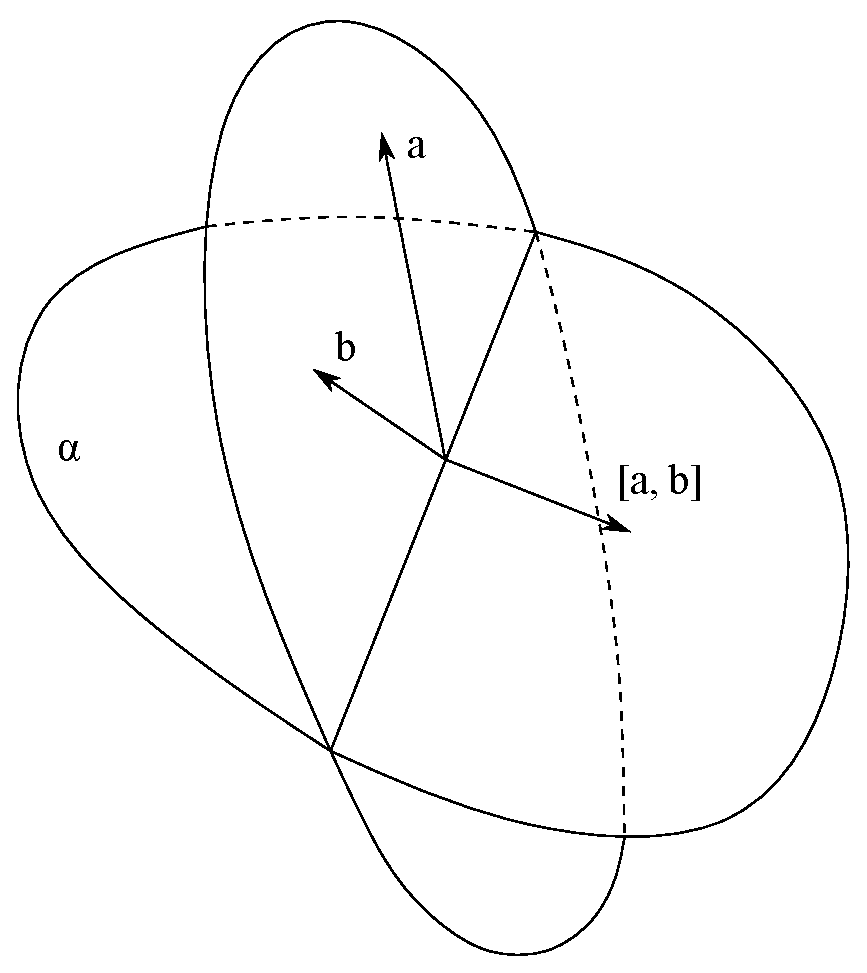
\includegraphics[width=0.5\columnwidth]{awkward-atom-or-a-pair-of-eggs}
      
      \caption{$\alpha$~---~плоскость, где лежат $[\bds a, \bds b]$, $[\bds b, \bds c]$ и $[\bds c, \bds a]$.}
      \label{fig:awkward-atom-or-a-pair-of-eggs}
    \end{figure}
    
    Рассмотрим пару векторов $\bds a$ и $\bds b$.
    Их векторное произведение $[\bds a, \bds b]$ лежит в $\alpha$ и перпендикулярно плоскости, где лежат $\bds a$ и $\bds b$ (пока считаем, что векторы $\bds a$, $\bds b$, $\bds c$ неколлинеарны).
    Таким образом, векторы $\bds a$ и $\bds b$ лежат в плоскости, перпендикулярной $\alpha$.
    Аналогично и с парами векторов $\bds a$, $\bds c$ и $\bds b$, $\bds c$.
    Все три такие плоскости попарно пересекаются хотя бы по одной прямой (например, плоскости векторов $\bds a$, $\bds b$ и векторов $\bds a$, $\bds c$ пересекаются хотя бы по прямой, содержащей вектор $\bds a$: векторы $\bds a$, $\bds b$, $\bds c$ изначально отложены от одной точки).
    Таким образом, если все три описанные плоскости совпадают, то вектора $\bds a$, $\bds b$, $\bds c$ лежат в ней, а потому компланарны.
    Если же плоскости не совпадают, а пересекаются попарно по одной прямой, то все три вектора $\bds a$, $\bds b$, $\bds c$ оказываются перпендикулярными $\alpha$, а потому параллельными.
    То есть в этом случае векторы $\bds a$, $\bds b$, $\bds c$ не только компланарны, но и коллинеарны.
    Но в процессе решения было сделано предположение о том, что $\bds a$, $\bds b$, $\bds c$ неколлинеарны, поэтому такой случай отпадает.
    
    Пусть теперь хотя бы один вектор из тройки $[\bds a, \bds b]$, $[\bds b, \bds c]$, $[\bds c, \bds a]$ равен нулевому вектору.
    Тогда либо хотя бы два вектора из трёх $\bds a$, $\bds b$, $\bds c$ коллинеарны, а потому все три они компланарны.
    Либо хотя бы один вектор из трёх $\bds a$, $\bds b$, $\bds c$ равен нулевому вектору, а потому все три снова компланарны.
  
    \bigskip
    
    \emph{``Формульный''.}
    
    Рассмотрим линейную комбинацию
    \[
      \alpha \bds a + \beta \bds b + \gamma \bds c = \bds 0
    \]
    
    Умножим векторно обе части на $\bds a$ слева.
    Получим
    \[
      \beta \cdot [\bds a, \bds b] + \gamma \cdot [\bds a, \bds c] = \bds 0
    \]
    
    Аналогично, при умножении векторно слева обеих частей исходного уравнения на $\bds b$ и $\bds c$:
    \[
      \left\{
        \begin{aligned}
          &\alpha \cdot [\bds b, \bds a] + \gamma \cdot [\bds b, \bds c] = \bds 0\\
          &\alpha \cdot [\bds c, \bds a] + \beta \cdot [\bds c, \bds b] = \bds 0
        \end{aligned}
      \right.
    \]
    
    Складывая все три полученных уравнения, получаем
    \[
      (\beta - \alpha) \cdot [\bds a, \bds b] + (\gamma - \beta) \cdot [\bds b, \bds c] + (\gamma - \alpha) \cdot [\bds a, \bds c] = \bds 0
    \]
    
    Так как векторы $[\bds a, \bds b]$, $[\bds b, \bds c]$, $[\bds c, \bds a]$ линейно зависимы, то хотя бы один из коэффициентов $(\beta \hm- \alpha)$, $(\gamma \hm- \beta)$, $(\gamma \hm- \alpha)$ может быть отличен от нуля.
    Но в таком случае три коэффициента в исходном уравнении $\alpha$, $\beta$, $\gamma$ не совпадают, а потому все три не могут в данном случае быть равны нулю одновременно.
    То есть существует нетривиальная линейная комбинация $\alpha \bds a \hm+ \beta \bds b \hm+ \gamma \bds c$, равная нулевому вектору.
    Поэтому три вектора $\bds a$, $\bds b$, $\bds c$ компланарны.
  \end{solution}

  
  \begin{problem}[3.31]
    Решить систему векторных уравнений в пространстве
    \[
      \left\{
        \begin{aligned}
          (\bds x, \bds a) = p\\
          (\bds x, \bds b) = q\\
          (\bds x, \bds c) = s
        \end{aligned}
      \right.
    \]
    где векторы $\bds a$, $\bds b$ и $\bds c$ некомпланарны.
  \end{problem}
  
  \begin{solution}
    Сначала покажем, что если $\bds a$, $\bds b$ и $\bds c$ некомпланарны, то и $[\bds a, \bds b]$, $[\bds b, \bds c]$ и $[\bds a, \bds c]$ некомпланарны.
    Рассмотрим линейную комбинацию
    \[
      \alpha [\bds a, \bds b] + \beta [\bds b, \bds c] + \gamma [\bds c, \bds a] = \bds 0
    \]
    Умножим обе части скалярно на $\bds b$ слева.
    Получим
    \[
      \gamma (\bds b, \bds c, \bds a) = \bds 0
    \]
    Откуда $\gamma \hm= 0$, так как $\bds a$, $\bds b$ и $\bds c$ некомпланарны (и их смешанное произведение отлично от нуля).
    Аналогично $\alpha \hm= 0$ и $\beta \hm= 0$.
    Поэтому три вектора $[\bds a, \bds b]$, $[\bds b, \bds c]$ и $[\bds a, \bds c]$ также некомпланарны.
    
    \bigskip
    
    Введём понятие \emph{взаимного базиса}.
    
    \begin{definition}
      Пусть есть базис $e \hm= (\bds e_1, \bds e_2, \bds e_3)$.
      Тогда взаимный базис $e^* \hm= (\bds e_1^*, \bds e_2^*, \bds e_3^*)$ определяется как
      \begin{equation}\label{eq:dual-basis}
        \left\{
          \begin{aligned}
            &\bds e_1^* = \frac{[\bds e_2, \bds e_3]}{(\bds e_1, \bds e_2, \bds e_3)}\\
            &\bds e_2^* = \frac{[\bds e_3, \bds e_1]}{(\bds e_1, \bds e_2, \bds e_3)}\\
            &\bds e_3^* = \frac{[\bds e_1, \bds e_2]}{(\bds e_1, \bds e_2, \bds e_3)}
          \end{aligned}
        \right.
      \end{equation}
    \end{definition}
    
    По доказанному ранее, $e^*$ в самом деле базис (три линейно независимых вектора в пространстве).
    Также можно заметить, что $(\bds e_i, \bds e_i^*) \hm= 1$ и $(\bds e_i, \bds e_j^*) \hm= 0$ при $i \hm{\not=} j$ (поэтому базис $e^*$ также называют биортогональным к базису $e$)\footnote{Эти свойства на самом деле и определяют взаимный базис в общем случае $\RR^n$ (\href{https://en.wikipedia.org/wiki/Dual\_basis}{en.wikipedia.org/wiki/Dual\_basis}).}.
    
    \bigskip
    
    Возвращаясь к задаче, разложим вектор $\bds x$ по взаимному к $\{\bds a, \bds b, \bds c\}$ базису $\{\bds a^*, \bds b^*, \bds c^*\}$:
    \[
      \bds x = x_1^* \bds a^* + x_2^* \bds b^* + x_3^* \bds c^*
    \]
    
    Умножая скалярно по очереди на $\bds a$, $\bds b$, $\bds c$ и пользуясь свойством ``биортогональности'' взаимного базиса, получаем
    \[
      \left\{
        \begin{aligned}
          &(\bds x, \bds a) = x_1^*\\
          &(\bds x, \bds b) = x_2^*\\
          &(\bds x, \bds c) = x_3^*
        \end{aligned}
      \right.
    \]
    
    То есть числа $p$, $q$ и $s$, данные в условии, есть компоненты вектора $\bds x$ во взаимном к $\{\bds a, \bds b, \bds c\}$ базисе, векторы которого вычисляются по (\ref{eq:dual-basis}).
  \end{solution}
  
  
  
  \begin{problem}[3.22(1)]
    Три некомпланарных вектора $\bds a$, $\bds b$, $\bds c$ отложены из одной точки.
    Найти объём треугольной призмы, основание которой построено на $\bds a$ и $\bds b$, а боковое ребро совпадает с вектором $\bds c$.
  \end{problem}
  
  \begin{solution}
    \begin{figure}[h]
      \centering
      
      \includegraphics[width=0.5\columnwidth]{triangular-prism}
      
      \caption{Треугольная призма, построенная на $\bds a$, $\bds b$ и $\bds c$.}
      \label{fig:triangular-prism}
    \end{figure}
    
    Объём призмы $V'$ равен произведению площади основания на высоту (\ref{fig:triangular-prism}).
    В основании треугольник~---~площадь которого в два раза меньше площади параллелограмма, построенного на тех же векторах $\bds a$ и $\bds b$.
    То есть объём призмы ищется аналогично объёму $V$ параллелепипеда, построенного на $\bds a$, $\bds b$, $\bds c$, только площадь основания в два раза меньше.
    Поэтому и
    \[
      V' = \frac{1}{2} V = \frac{\bigl|(\bds a, \bds b, \bds c)\bigr|}{2}
    \]
    
    Задача решена.
    Нашли объём, не находя ни высоты, ни площади основания.
    
    \bigskip
    
    \emph{Отступление.}
    
    Но как можно бы было найти вектор $\bds c_{\perp}$, по модулю равный высоте призмы и перпендикулярный основаниям?
    Вектор $\bds c$ можно представить в виде суммы двух векторов, один из которых параллелен плоскости основания призмы, а другой перпендикулярен плоскости основания.
    В свою очередь, компоненту $\bds c$, параллельную основаниям, можно разложить по векторам $\bds a$ и $\bds b$ (которые, как неколлинеарные вектора, образуют базис на плоскости).
    Получаем
    \[
      \bds c = \alpha \bds a + \beta \bds b + \bds c_{\perp}
    \]

    Если умножить полученное уравнение скалярно на $\bds a$ и на $\bds b$ (по очереди), то получим систему
    \[
      \left\{
        \begin{aligned}
          &(\bds c, \bds a) = \alpha (\bds a, \bds a) + \beta (\bds b, \bds a)\\
          &(\bds c, \bds b) = \alpha (\bds a, \bds b) + \beta (\bds b, \bds b)
        \end{aligned}
      \right.
    \]
    из которой уже можно найти $\alpha$ и $\beta$, например, по правилу Крамера, если определитель системы отличен от нуля:
    \[
      \Delta = \begin{vmatrix}
        (\bds a, \bds a) & (\bds a, \bds b)\\
        (\bds a, \bds b) & (\bds b, \bds b)
      \end{vmatrix}
      = |\bds a|^2 |\bds b|^2 - |\bds a|^2 |\bds b|^2 \cos^2 \angle{(\bds a, \bds b)}
      = \bigl|[\bds a, \bds b]\bigr|^2
      \not= 0
    \]
    так как векторы $\bds a$ и $\bds b$ неколлинеарны.
    А вообще, определитель
    \[
      \begin{vmatrix}
        (\bds a, \bds a) & (\bds a, \bds b)\\
        (\bds a, \bds b) & (\bds b, \bds b)
      \end{vmatrix}
    \]
    называется \emph{определителем Грама\footnote{\href{https://en.wikipedia.org/wiki/Gramian\_matrix}{en.wikipedia.org/wiki/Gramian\_matrix}.}} системы векторов $\bds a$ и $\bds b$.
    Из решения видно, что отличие от нуля определителя Грама системы векторов является \emph{критерием линейной независимости} этой системы векторов (чтобы коэффициенты разложения любого вектора по этой системе определялись однозначно~---~в нашем случае коэффициенты разложения компоненты $\bds c$, параллельной основанию призмы, по векторам $\bds a$ и $\bds b$).
    
    Возвращаясь к вектору $\bds c_{\perp}$, то при найденных $\alpha$ и $\beta$ он получается равным
    \[
      \bds c_{\perp} = \bds c - \alpha \bds a - \beta \bds b
    \]
  \end{solution}
\end{document}
